\documentclass[12pt]{article}

\title{Symbolic Logic HW 4}
\author{Tyler Tracy}

\usepackage{amsmath}
\usepackage{amssymb}
\usepackage{graphicx}
\graphicspath{ {./imgs/} }

\begin{document}

\section*{Solution to Problem 1}

\subsection*{Part A}

\includegraphics[width=\textwidth]{1a}

\subsection*{Part B}

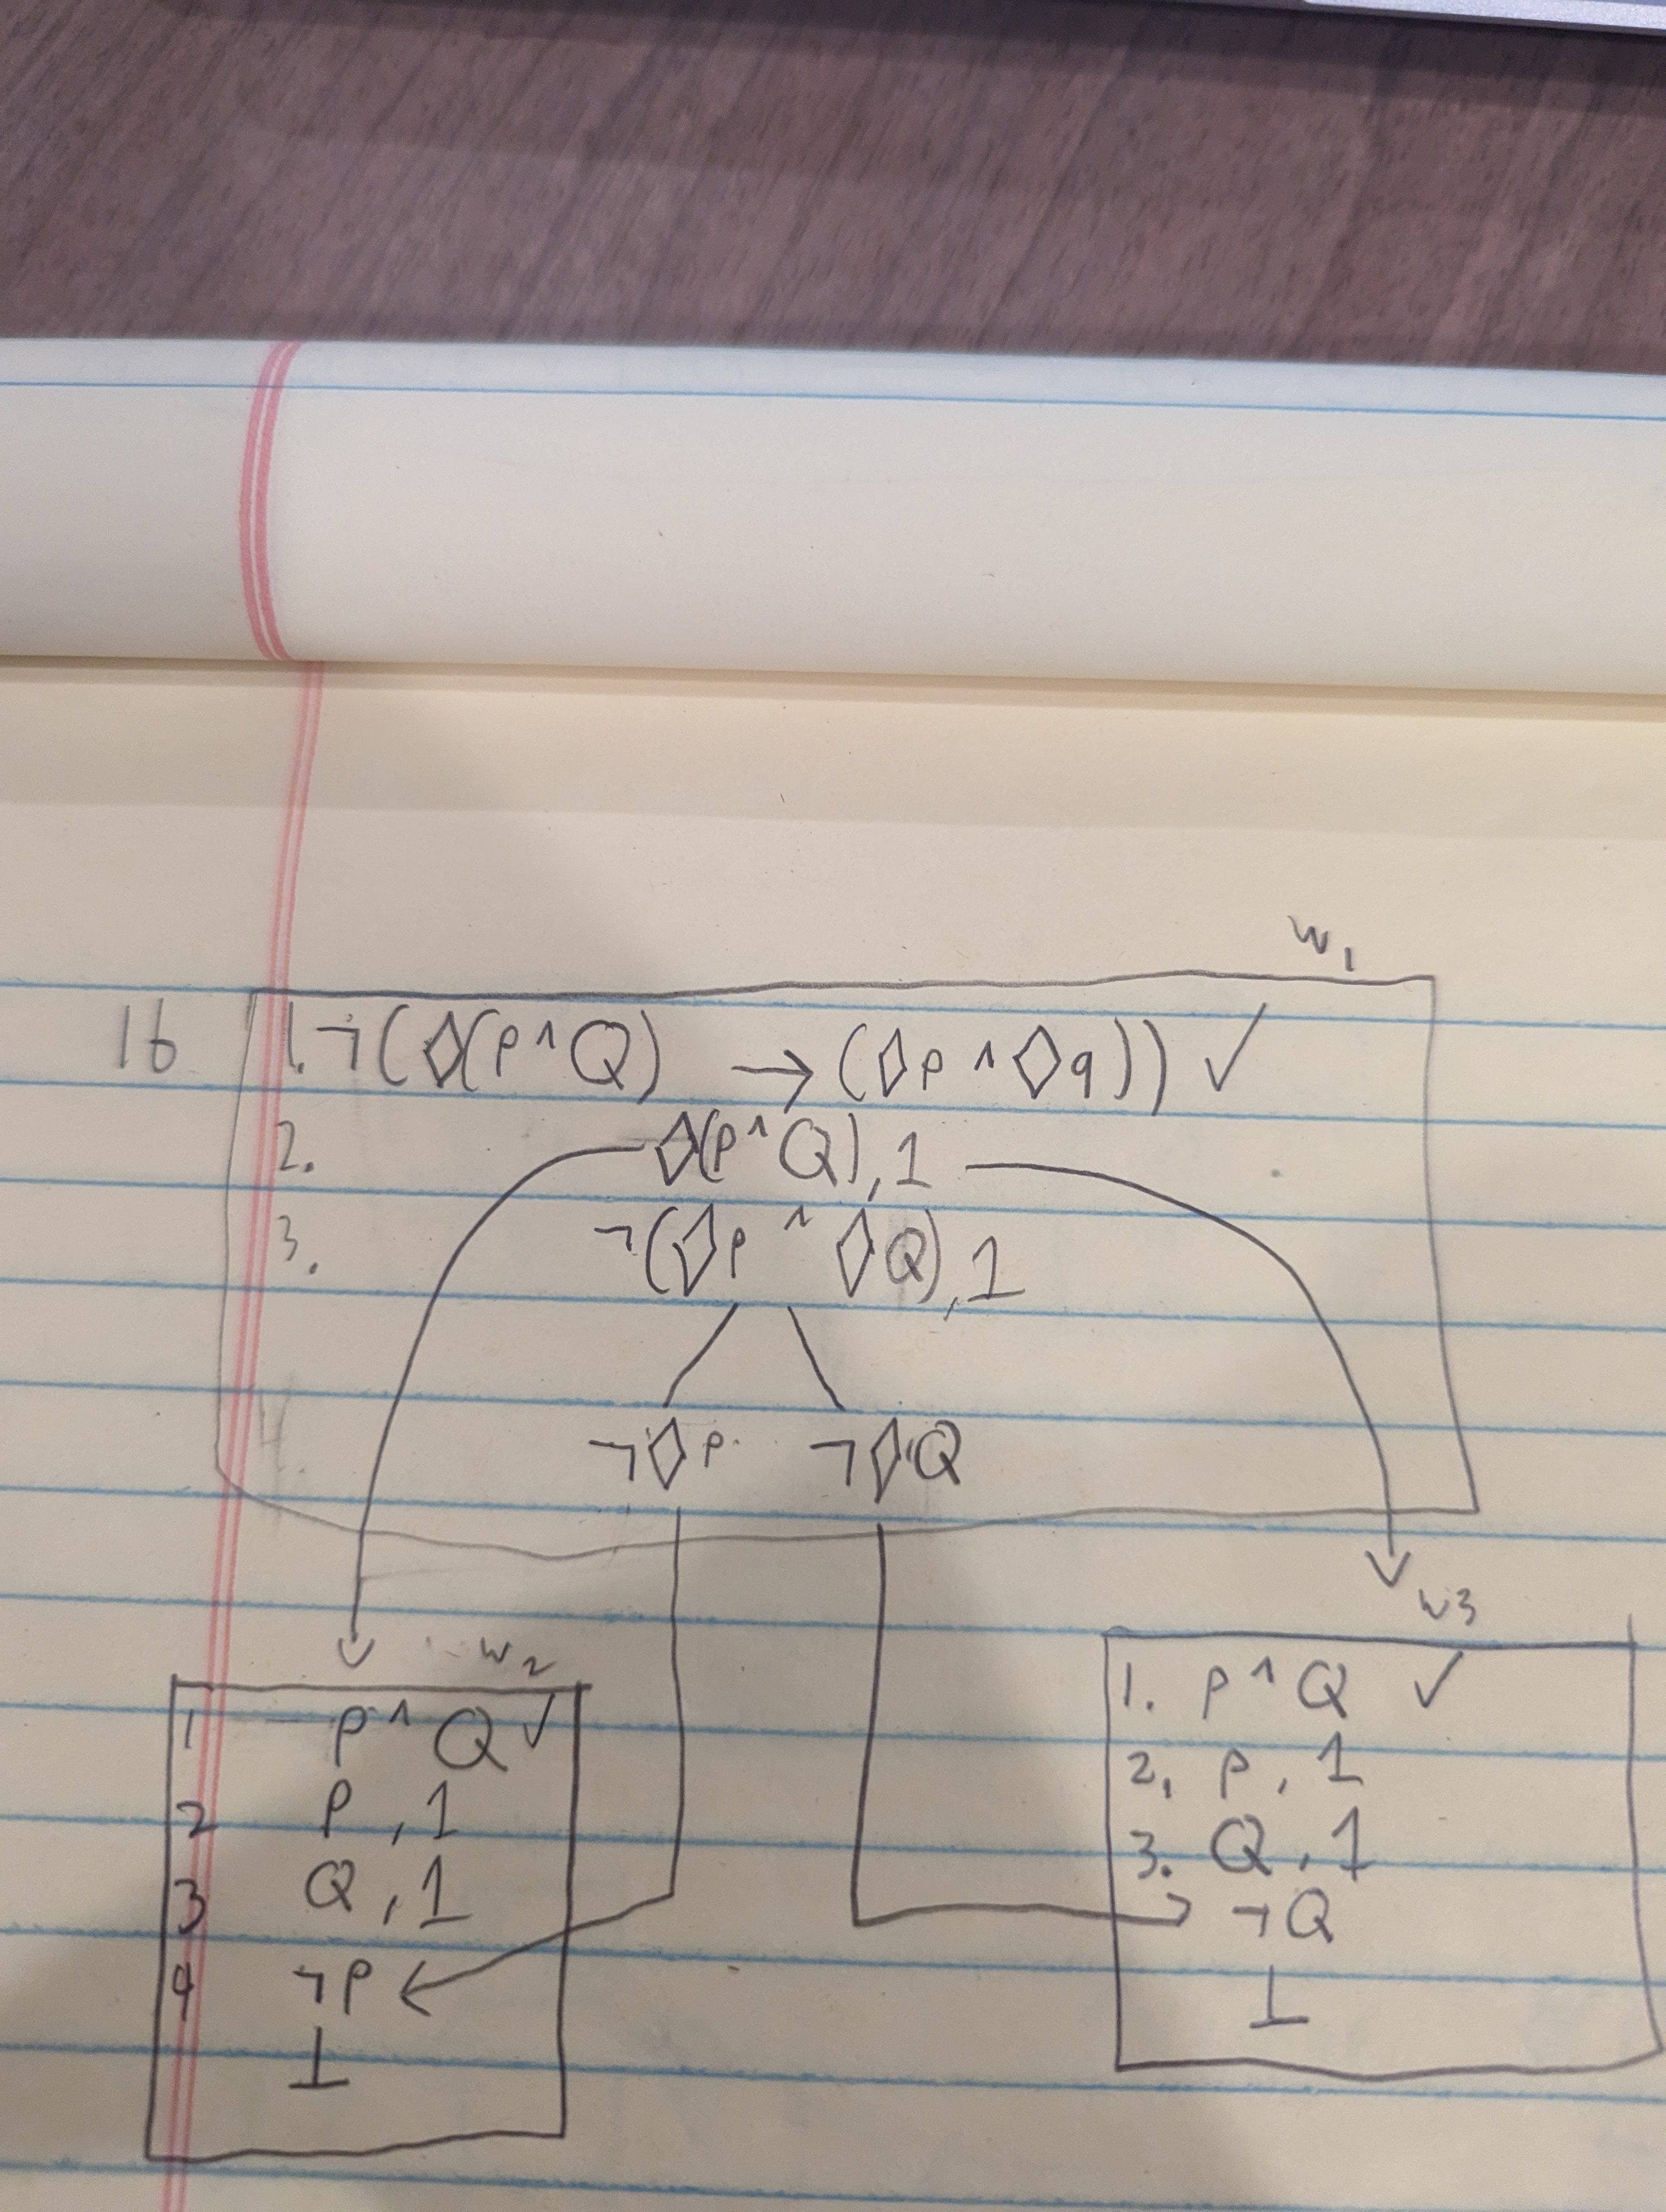
\includegraphics[width=\textwidth]{1b}

\section*{Solution to Problem 2}

Let the domain = the set of people. Symbolize the following sentences, using P = is a philosopher, W = is wise, Txy = x teaches y, Lxy = x learns from y, s = Socrates, p = Plato. 

\begin{itemize}
    \item Everyone learns from someone \\
        $\forall x \exists y Lxy$
    \item Someone learns from everyone \\
        $\exists x \forall y Lxy$
    \item Someone learns from everyone who learns from them \\
        $\exists x \forall y (Lyx \rightarrow Lxy)$
    \item Someone learns from no-one \\
        $\exists x \forall y \neg Lxy$
    \item Everyone has someone they learn from who also learns from them \\
        $\forall x \exists y (Lxy \land Lyx) $
    \item Some wise people aren’t philosophers, but all philosophers are wise \\
        $(\forall x Px \rightarrow Wx) \land (\exists y Wy \land \lnot Py)$
    \item Anyone who was taught by Socrates was wise  \\
        $\forall x Tsx \rightarrow Wx$
    \item If everyone is a philosopher, then Socrates is a philosopher \\
        $(\forall x Px) \rightarrow Ps$
    \item If anyone is a philosopher, then Socrates is a philosopher \\
        $(\exists x Px) \rightarrow Ps$
    \item Anyone who is taught by Socrates learns from Socrates \\
        $\forall x (Tsx \rightarrow Lxs)$
    \item Whoever learns from Plato, learns from Socrates \\
        $\forall x (Lxp \rightarrow Lxs)$
    \item If no-one is wise, then no-one is a philosopher \\
        $(\lnot \exists x Wx) \rightarrow (\lnot \exists x Px) $
    \item If everyone is taught by a philosopher, then everyone will be wise\\
        $(\forall x \exists y (Tyx \land Py)) \rightarrow (\forall x Wx)$
\end{itemize}


\section*{Solution to Problem 3}


\subsection*{Part A}

$\forall y Lya \rightarrow \forall y Lay, Lba, \therefore Lab$

If everyone loves Alma then Alma loves everyone. Baron loves Alma. Therefore Alma loves Baron. 

This is not true because only Baron loves Alma, not everyone. 

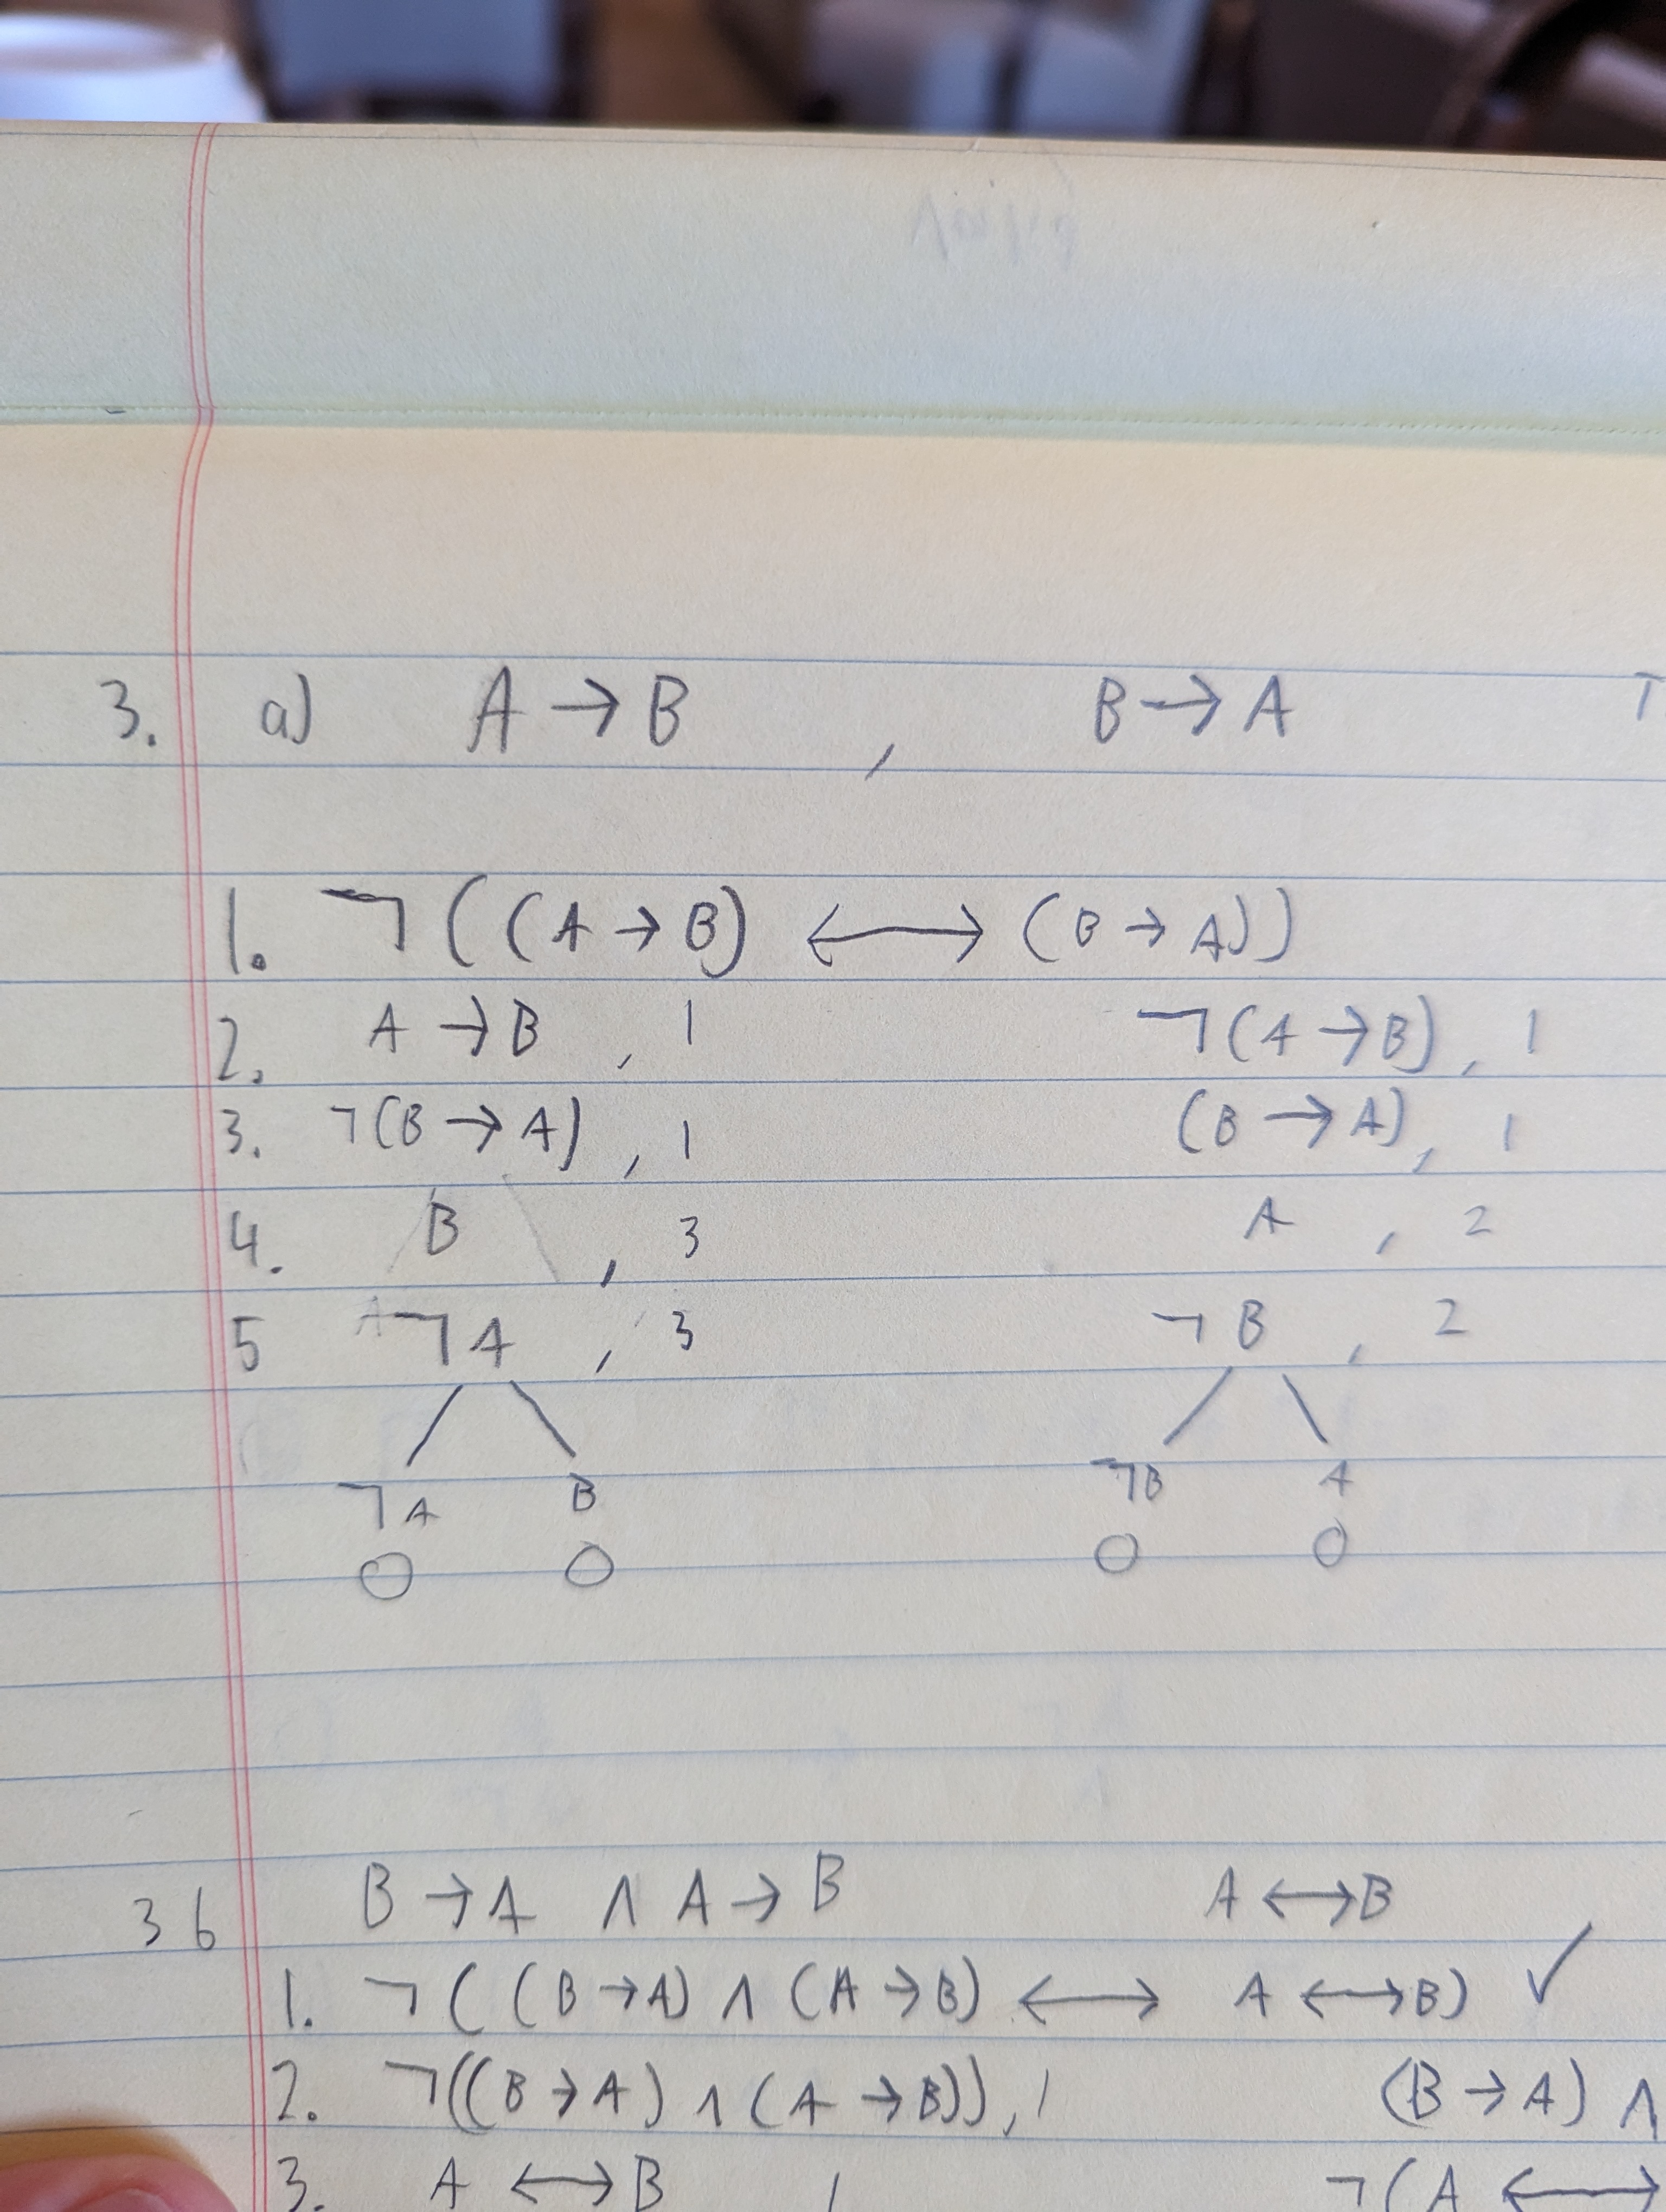
\includegraphics[width=\textwidth]{3a}

\subsection*{Part B}
$\forall x \forall y (Lxy \rightarrow Lyx), Lba, \therefore Lab$

If someone someone loves someone, then that person loves them back. Baron loves Alma. Therefore Alma loves Baron.

This is true, Baron loves Alma, so Alma must love Baron back. 

\includegraphics[width=\textwidth]{3b}

\subsection*{Part C}
$\exists y \forall x Lxy \therefore \exists x \exists y(Lxy \land Lyx)$

There is someone who is loved by everyone. Therefore there is someone who loves and is loved by someone.

This is true. The someone who is loved by everyone loves themself, so they love and are loved. 

\includegraphics[width=\textwidth]{3c}

\subsection*{Part D}

$\exists x \forall y (Lxy \rightarrow Lyx), \forall x Lxb \therefore \forall x Lbx$

There is someone who is loved by everyone they love. Everyone one loves Baron. Thus Baron loves everybody.

This is false, the person who is loved by everyone they love that could be someone different than Baron. 

\includegraphics[width=\textwidth]{3d}

\section*{Solution to Problem 4}

\includegraphics[width=\textwidth]{4}

This tree produces an infinite chain of instances of $Lxy \land Gyx$. $x$ and $y$ will never be the same value so it will go on forever producint an infinite domain never closing the tree. The existiential is true in just the case of $Laa$ and $Gaa$ but not for all $x$. Since the tree never closes and will never produce a variable that makes it close, the argument is invalid. 

\section*{Solution to Problem 6}

 In performing the tree test in quantificational logic, a tree has not been completed until either 
 (i) it closes, or 
 (ii) in each open branch, you have performed UI on each universal generalization in that 
branch using every name that appears in that branch. Suppose we relaxed this requirement in the following way: You are only required to perform UI using one name in each branch to complete the tree. 

In each case: if you think the tree test would still be adequate, informally explain why;  If you think the tree test would  be inadequate in the relevant respect, give a counterexample i.e., a tree constructed in conformity with the modified procedure that demonstrates that the tree test lacks the relevant property.


\subsection*{Would the modified tree test be sound}

I think the test would still be sound. Since we are doing the same procedure but just less steps, then any tree that was invalid and open would still be invalid and open. This doesn't add more ways to close trees so no tree would be closed by this modified test that wasn't closed by the true tree test.  

\subsection*{Would the modified tree test be complete}

It would not be complete. Here is a valid argument that the tree test leaves open. 

\includegraphics[width=\textwidth]{6b}

\section*{Solution to Problem 7}





\subsection*{Part A}
A sentence of form $p \lor q$ is a tautology only if at least one of p and q is a tautology 

This is false. The case where $q = \lnot p$ would make $p \lor q$ always true but neither $p$ nor $q$ is always true. 

\subsection*{Part B}

If $\{p1, p2, …, pn\}$ is inconsistent, then $\{p1, p2, …, pn \} \models q$, for arbitrary q. 

This is true. An inconsistent set can imply anything to be true, so it can imply any q to be true. 

\subsection*{Part C}
If $p \land q$ is a contradiction, then $p \land \lnot q$ is a tautology. 

This is false. Imagine that $q = \lnot p$. This means $p \land \lnot p$ is a contradiction. But $p \land p$ is not a tautology. It is false when p is true. 

\subsection*{Part D}
If $\Gamma \bigcup \{p\} \models q$, then $\Gamma \models p \rightarrow q$ 

This is false. Image $\Gamma = \{ q \}$. $\Gamma \bigcup \{p\} \models q$ is true. But $\Gamma \models p \rightarrow q$ is not true. 



\end{document}
